% !TEX root =  master.tex
\chapter{Data}\label{chapter:data}

\section{NIH Data}\label{data:nih}
\sectionauthor{Written by Tobias Richstein}

The first of the datasets that we used to train our models comes from the \acf{NIH}, a division of the U.S. Department of Health, and is a collection of over 100 thousand chest X-ray images by over 30 thousand patients presented by \citeauthor{wang_chestx-ray8_2017} in \autocite{wang_chestx-ray8_2017}. This dataset was published in 2017 and is therefore not concerned with COVID-19 patients at all. Rather it consists of images depicting 14 different illnesses and images of healthy patients. The authors claim that there is a large amount of data in the form of patient X-rays and corresponding findings available in hospital's archiving systems but that these have not been properly consolidated and catalogued across multiple hospitals and states before. The authors also claim that the findings are mostly embedded in sentences making them not easily machine-readable.

To overcome these issues, the authors collected the images from different hospitals and used natural language processing to extract the medical findings from the written reports associated with the images. In the initial dataset this included eight different illnesses: Atelectasis, Cardiomegaly, Effusion, Infiltration, Mass, Nodule, Pneumonia and Pneumothorax as well as images with no finding at all. Later, the dataset was updated to the 15 class form (14 illnesses and no findings) that we use for our project to also include Consolidation, Edema, Emphysema, Fibrosis, Pleural Thickening and Hernia as findings. The class distribution can be seen in figure \vref{fig:nih_classes} where it is clear that the classes are very disproportionally represented. There is a total of $141,537$ diagnoses, meaning each image has an average of roughly $1.26$ labels associated. This number is skewed however since if anything is found then the average goes up to $1.56$ since no finding always means that only this one label is attached to a record.

\begin{figure*}
	\centering
	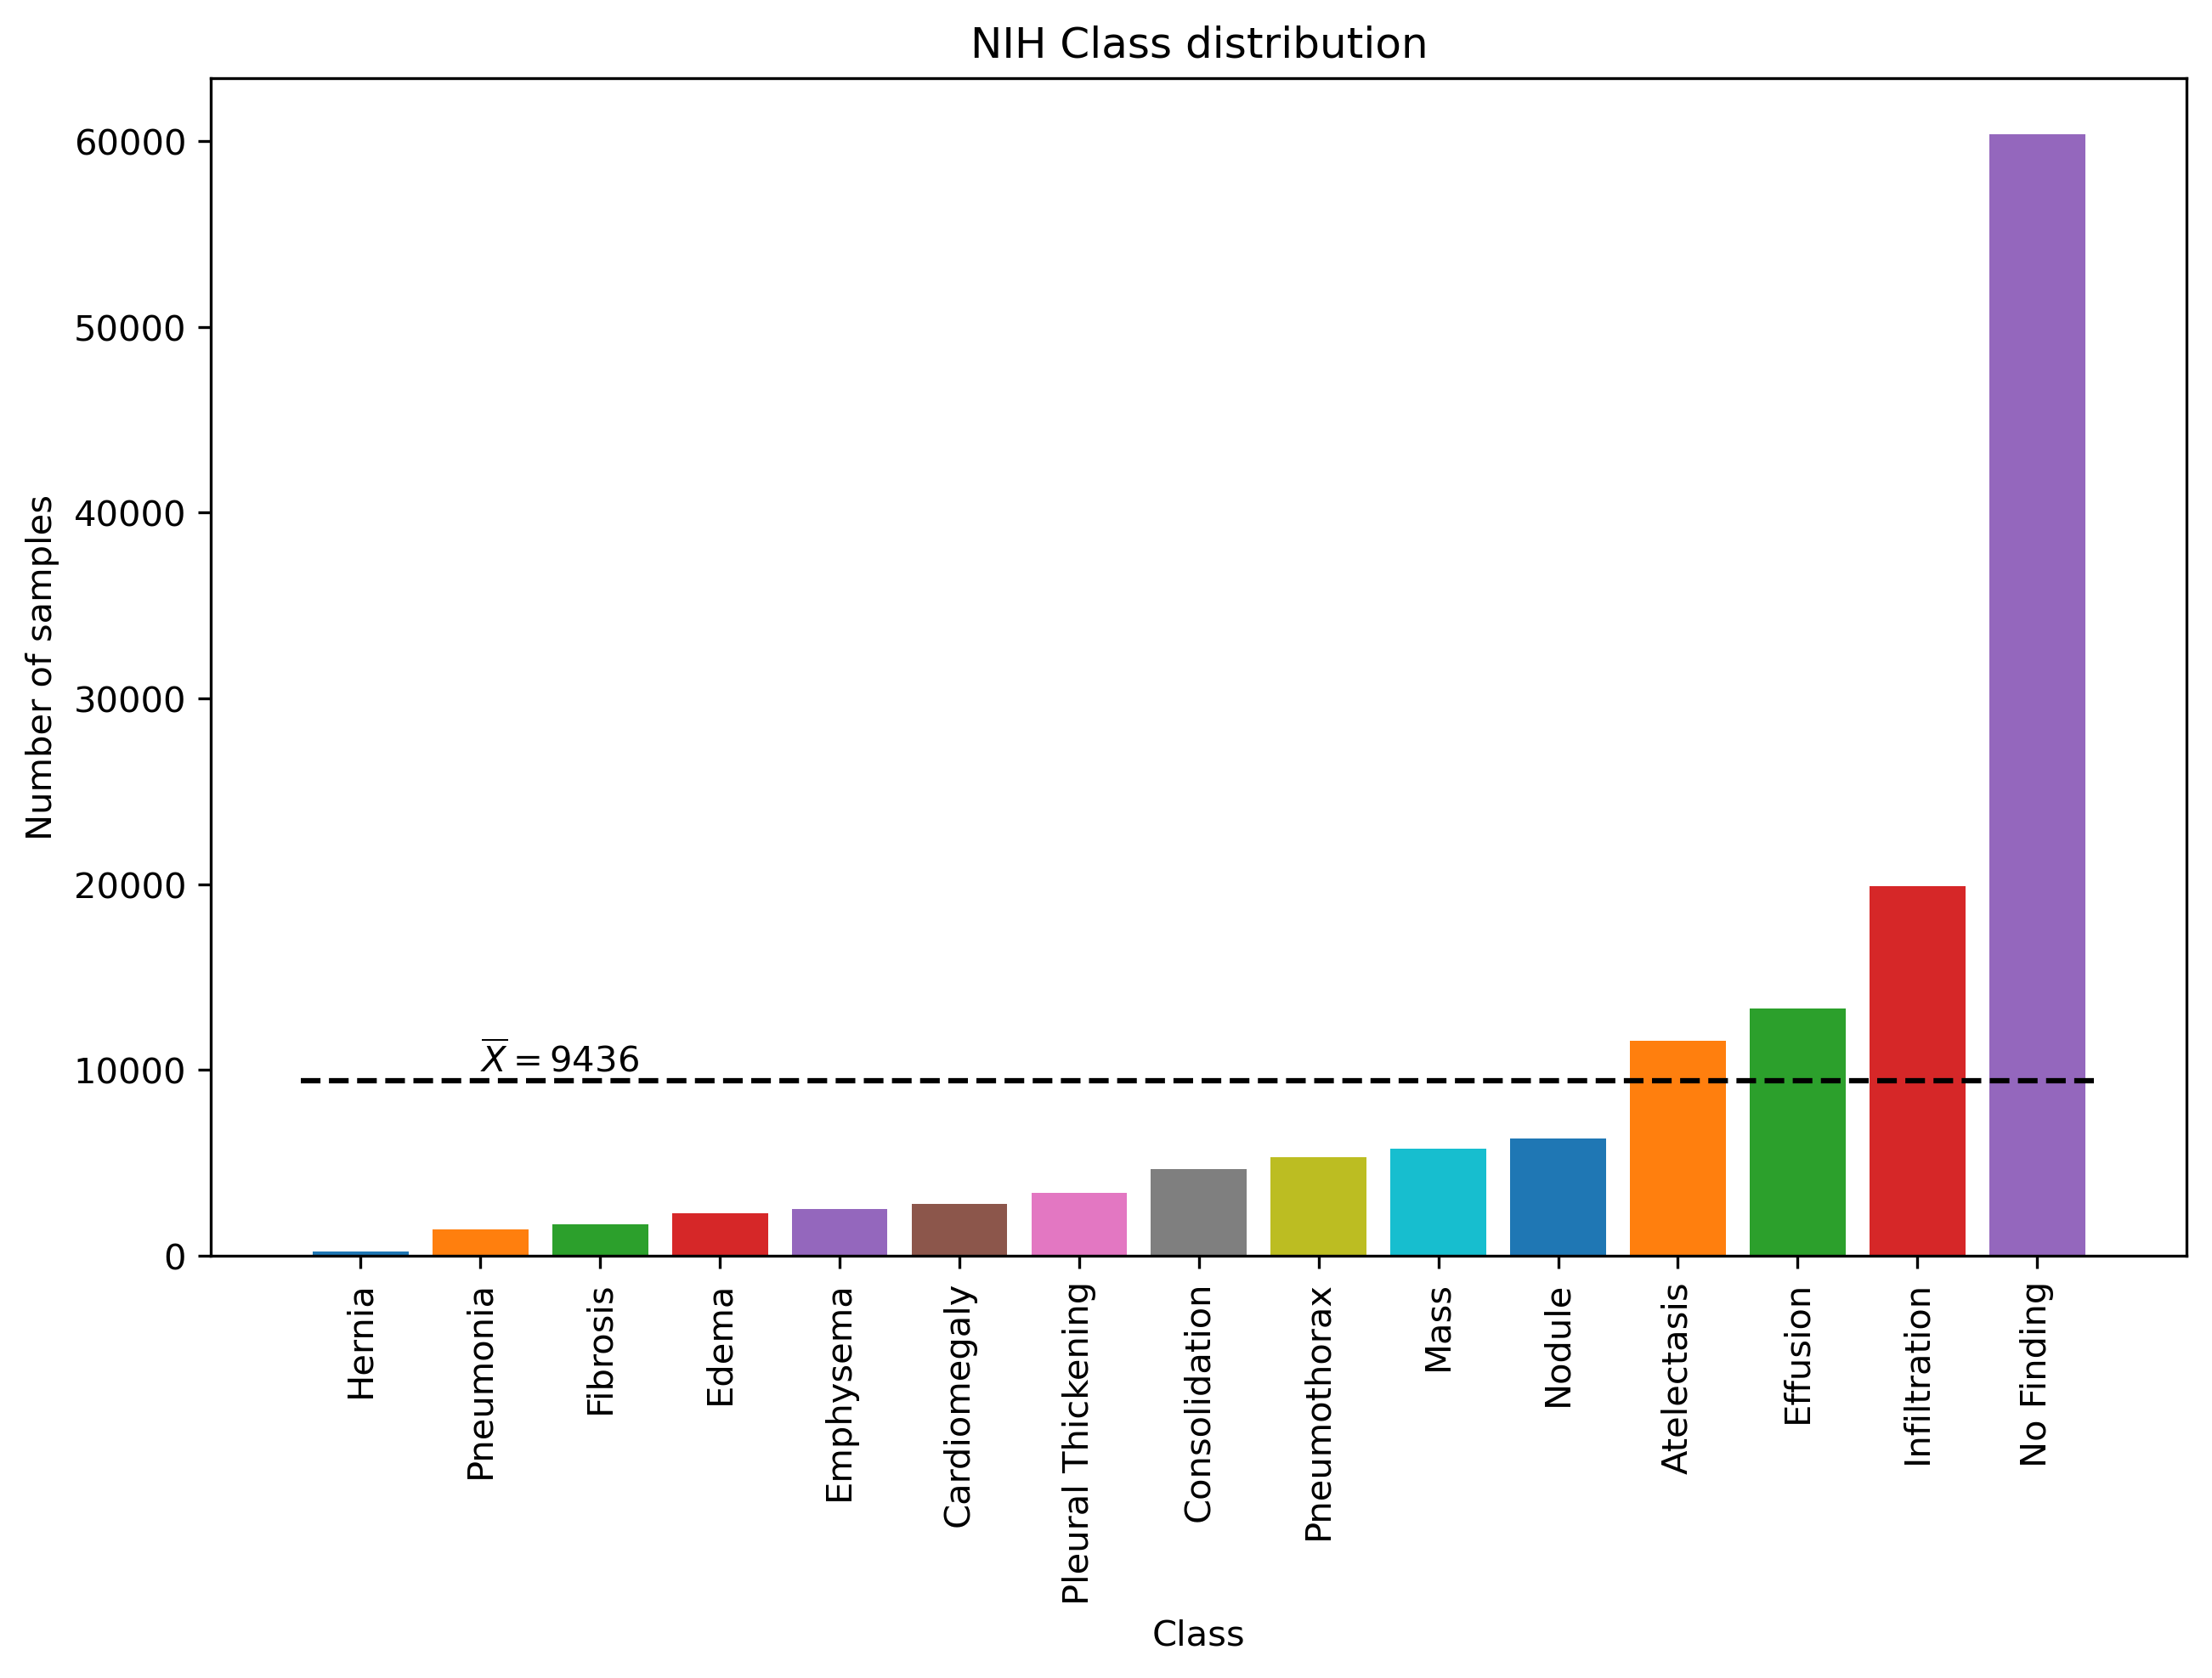
\includegraphics[width=.8\linewidth]{img/nih_class_distribution.png}
	\caption{Class distribution in the NIH dataset}
	\label{fig:nih_classes}
\end{figure*}

The images in the dataset are given in the PNG format and are all sized $1024 \times 1024$ and with RGB color channels. The dataset does have roughly six thousand entries for bounding boxes for some of the images but those are not really of use to us since there are so few and also because the value of this dataset lies somewhere else for us: The training of our backbone network for one of the object detection networks (more on that in section \vref{chapter:rcnn}). We can use this dataset to train the backbone on images that are roughly within the problem domain that we actually want to tackle so that the feature vectors that it produces are valuable to the actual object detection network. 

\section{RSNA Data}\label{data:rsna}
\sectionauthor{Written by Julian Seibel}

Similar to the pretraining of the Faster \ac{R-CNN} backbone on the above described NIH dataset, we use the RSNA dataset \autocite{RSNAKaeggle} originally published as part of a two-stage Kaggle challenge in 2018. The dataset contains $30,227$ samples from $26,684$ different patients in form of $1024 \times 1024$ DICOM images. Despite the data was anonymized, for every patient there are meta-information available including sex, age and radiographic view. The images were labeled by radiologists from \ac{RSNA} and the Society of Thoracic Radiology. There are three mutual exclusive  labels possible (lung opacity, normal, no lung opacity/ not normal) whereas lung opacity describes a indicates evidence for pneumonia including also bounding box information for regions of interest in the format $(x_{min}, y_{min}, width, height)$. A positive image can contain multiple bounding boxes. Figure \ref{fig:rsna_classes} shows the class distribution for the \ac{RSNA} datasets. In total there are $9,555$ sample images that are labeled as positive and therefore come along with labeled regions in form of bounding boxes.

The objective of this challenge was to train a model that is capable of correct classification including also bounding box predictions for each positive case and a confidence score, indicating the model confidence for a single bounding box prediction. The final submissions were evaluated using \ac{IoU} based metrics to measure the overlap of predicted and ground truth boxes. Figure \ref{fig:rsna_sample} shows an image from the \ac{RSNA} dataset including ground truth boxes (green), possible predictions (reds-dashed) and corresponding \ac{IoU} values.

Since this challenge has a lot in common with the challenge we want to contribute to in this work and the image appearance is the exact same, namely DICOM images of chest X-rays, we decided to include this dataset as additional source for pretraining our models. In contrast to the \ac{NIH} dataset, the \ac{RSNA} data is rather small, but brings one major advantage with labels including ground truth bounding boxes for positive pneumonia cases which makes the data suitable for pretraining object detection models. With this, we also think there are semantic similarities in predicting pneumonia and COVID-19 regions, that we hope will positively affect our final model performance for ultimately detecting COVID-19 evidence. In detail, we used the positive cases for training our detection models to \enquote{introduce} the weights into the domain of medical X-ray chest images. For the meta-data of the patients however, we did not find any suitable purpose which is why we ignored this information in the further course of this work.

\begin{figure*}
	\begin{minipage}[b]{.65\linewidth} % [b] => Ausrichtung an \caption
		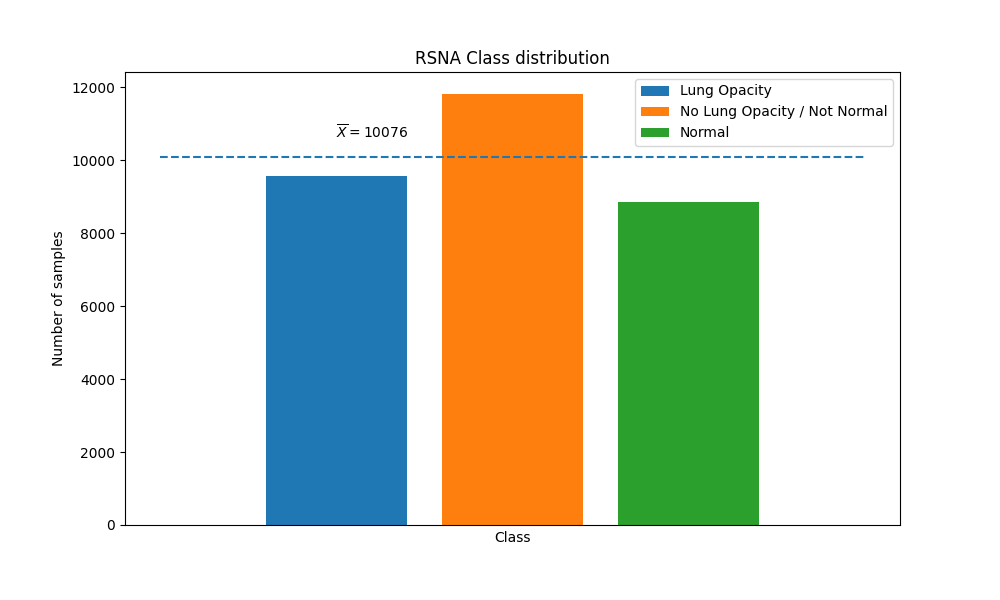
\includegraphics[width=\linewidth]{img/rsna_class_distribution.png}
		\caption{Class distribution in the RSNA dataset}
		\label{fig:rsna_classes}
	\end{minipage}
	\begin{minipage}[b]{.35\linewidth} % [b] => Ausrichtung an \caption
		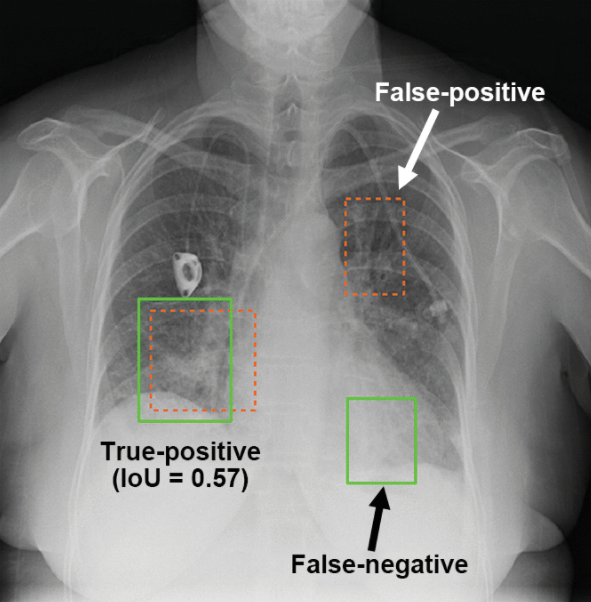
\includegraphics[width=\linewidth]{img/rsna_sample.png}
		\caption{Extracted from \autocite{rsnaSurvey}}
		\label{fig:rsna_sample}
	\end{minipage}
\end{figure*}

\section{SIIM COVID-19 Data}\label{data:siim}
\sectionauthor{Written by Torben Krieger}

// mini dicom intro ? study-series-image relation, transfer syntaxes --> uncompressed
// multi-label occurrence in train set

